\documentclass[11pt]{article}

\usepackage[margin=0.75in]{geometry}
\usepackage{amsfonts, amsmath, amssymb}
\usepackage[none]{hyphenat}
\usepackage{fancyhdr}
\usepackage{graphicx}
\usepackage{float}
\usepackage[nottoc, notlot, notlof]{tocbibind}
\usepackage{mathrsfs}
\usepackage{bm}
\usepackage[caption=false]{subfig}


% matlab code formatter
\usepackage{matlab-prettifier}
\usepackage{xcolor}
\definecolor{lbcolor}{rgb}{0.95,0.95,0.95}
% end of matlab formatter

\pagestyle{fancy}
\fancyhead{}
\fancyfoot{}
\fancyhead[L]{Signals and Systems (course 25742)}
\fancyhead[R]{Reza Nayeb Habib 401102694}
\fancyfoot[C]{\thepage}
\fancyfoot[R]{Sharif University of Technology}
\renewcommand{\footrulewidth}{1pt}
\parindent 0ex

\begin{document}
 
\begin{titlepage}
\begin{center}

\begin{figure}[H]
\begin{center}

\includegraphics[scale=0.4]{Fig/SUT.png}

\end{center}
\end{figure}

\huge{\textbf{Signals and Systems Software Homework Report}} \\ 
\vspace*{2cm}
\Large{\textbf{Instructor: Prof. Karbalaei}} \\
\vspace*{1cm}
\huge{\textbf{Sharif University of Technology}} \\
\line(1,0){500} \\ 
\Huge{\textbf{Project(Phase 1): Epileptic Seizure Prediction Using 
Spectral Entropy-Based Features of EEG}} \\
\line(1,0){500} \\
\vfill
\Large{By Reza Nayeb Habib}\\
\Large{Student ID\# 401102694} \\

\end{center}
\end{titlepage}

\tableofcontents
\thispagestyle{empty}
\clearpage
\setcounter{page}{1}


\section{Electrodes naming}
the naming convention of EEG is for showing different brain parts. \\
the numbering starts from low numbers when near the center of the brain and goes
higher when we get farther from the brain. the left side of head  has odd numbers
while the right side has even numbering. \\
F is for the frontal lobe of the brain so for example Fz is the central electrode. \\
P is for the Parietal lobe and O for Occipital lobe. also the left and right side
shown with T are for brains Temporal lobes. \\

\begin{figure}[H]
    \begin{center}
        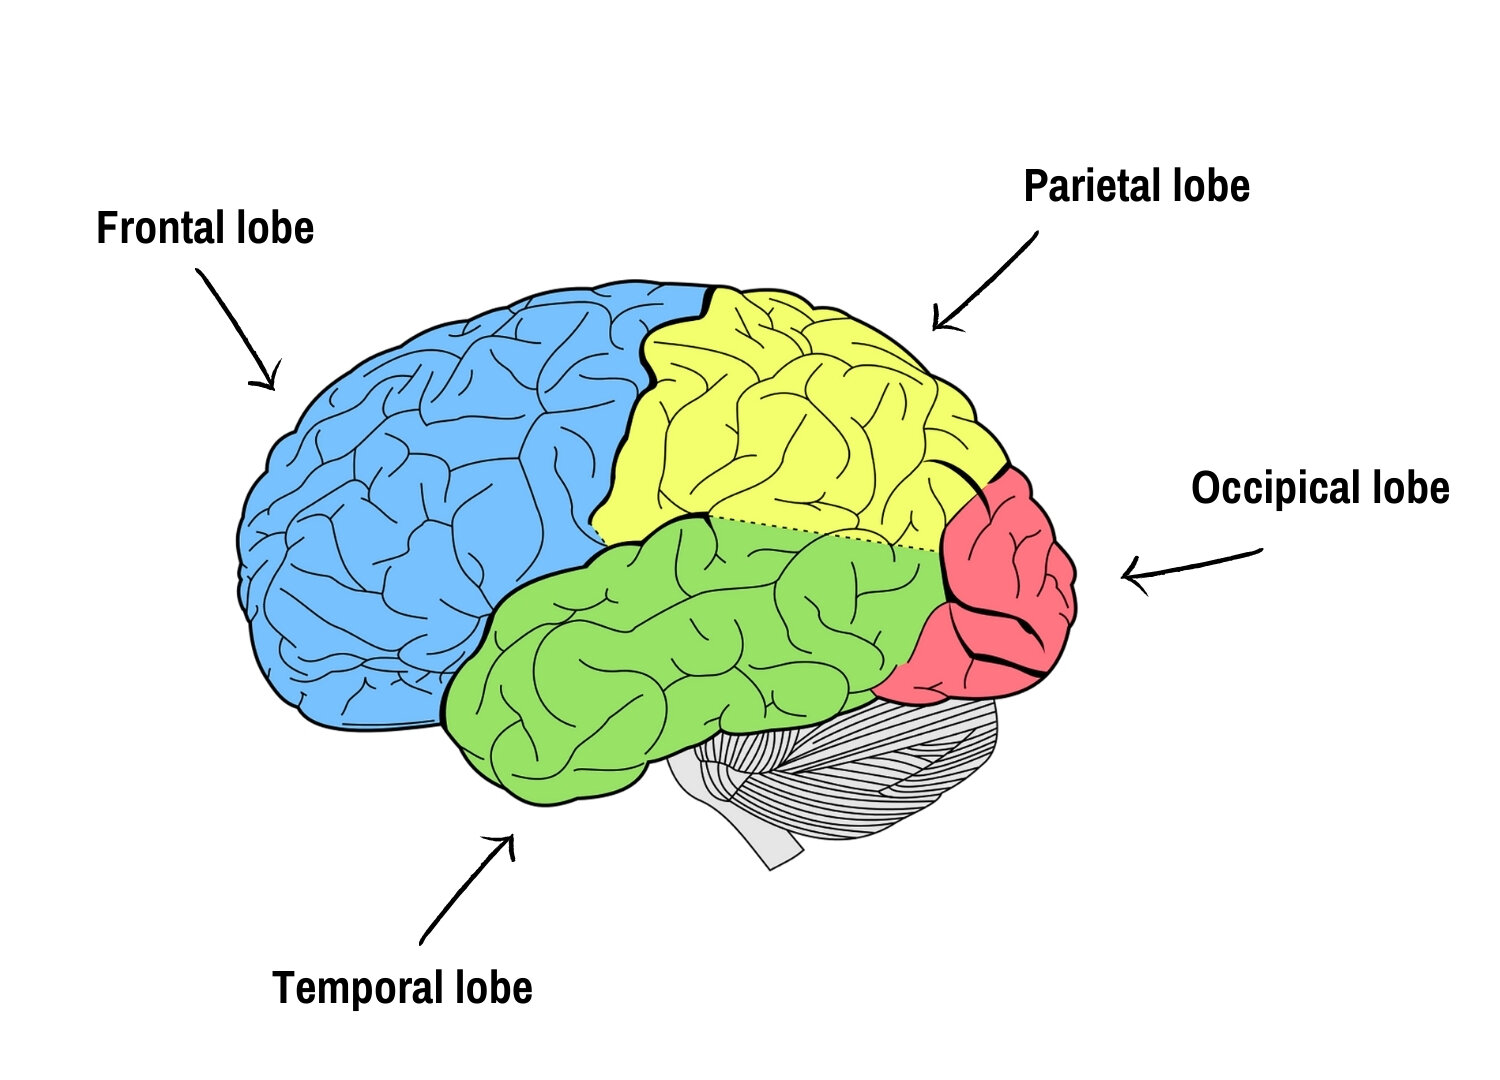
\includegraphics[scale=0.3]{Fig/brainLobes.jpg}
        \label{fig:brainLobes}
        \caption{brain Lobes}
    \end{center}
\end{figure}



\section{Frequency Bands of EEG}
\textbf{Determine the activities each frequency band is associated with:} \\

\begin{figure}[H]
    \begin{center}
        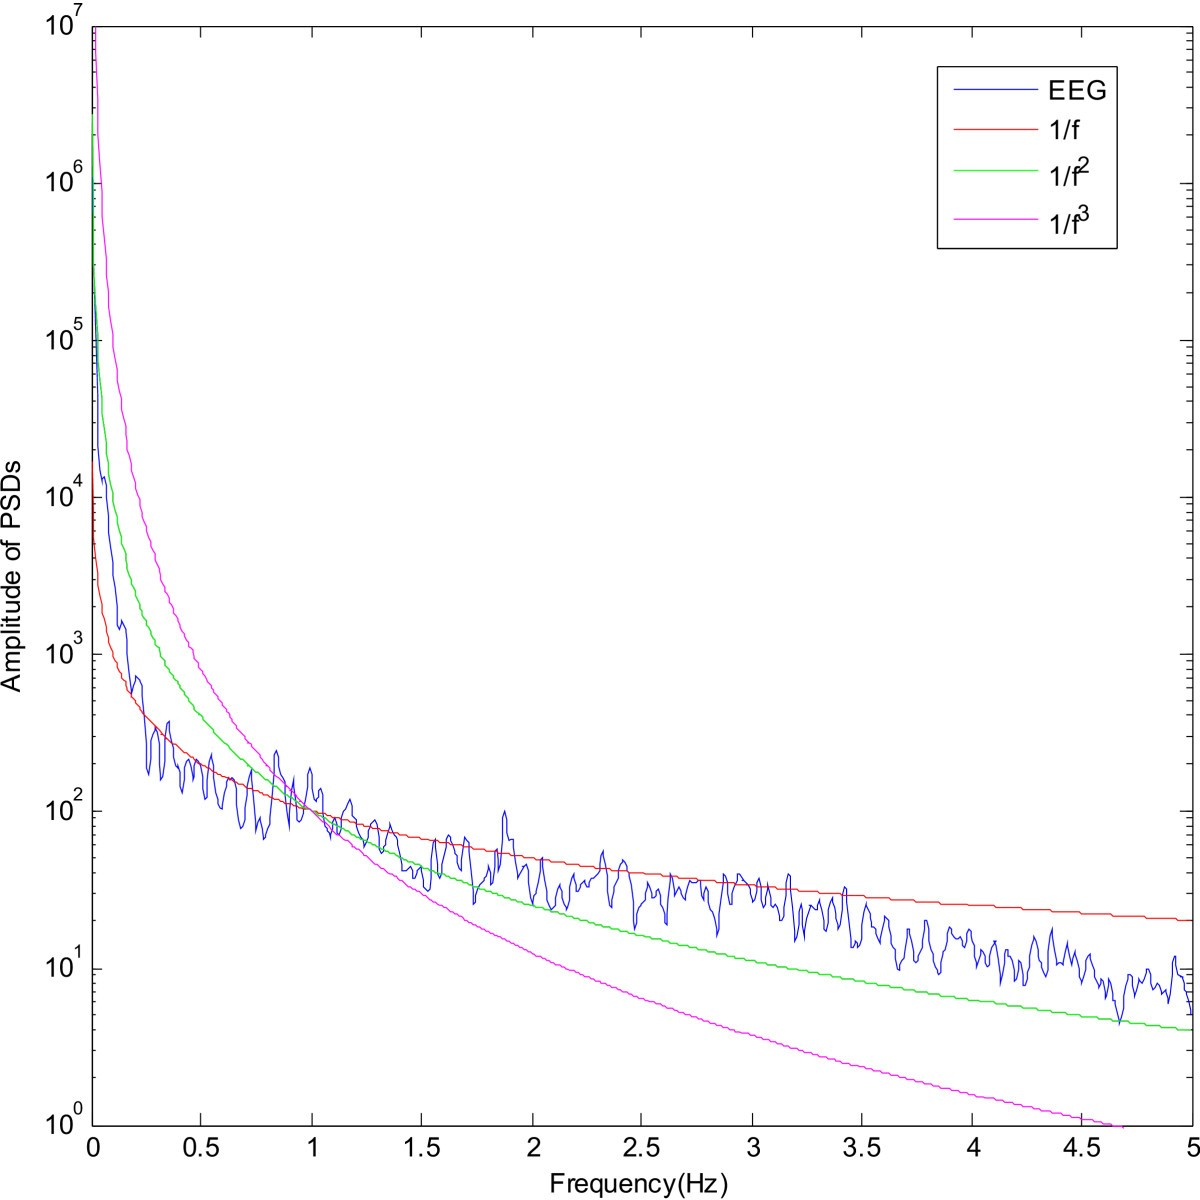
\includegraphics[scale=0.3]{Fig/brainSpectralPlot.jpg}
        \label{fig:frequencySpectrum}
        \caption{EEG frequency spectrum}
    \end{center}
\end{figure}

The EEG signal spectrum usually has a frequency spectrum with the shape $\frac{1}{f}$ 
(see the figure above), this means that we won't likely have 
any frequencies higher than 100Hz from the EEG and we usually consider frequency
content higher than 200Hz as noise. in figure 2 we can see different bands of
EEG signal and their conventional names. we will explain each frequency's corresponding brain functionality: \\

\begin{figure}[H]
    \begin{center}
        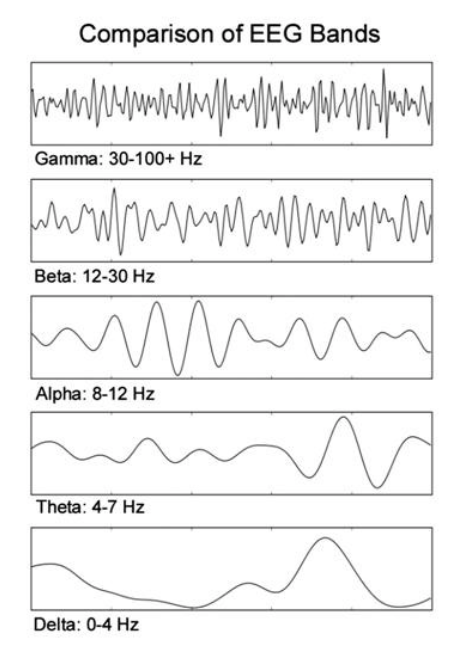
\includegraphics[scale=0.45]{Fig/EEGfreqs.png}
        \label{fig:EEGfreqBands}
        \caption{EEG frequency bands}
    \end{center}
\end{figure}

\textbf{Delta Waves: } these waves are typically generated when the brain is 
at rest or deep sleep. having too little may indicate poor sleep or Inability to rejuvenate body.
having too much of this frequency band's content may indicate Brain injuries, learning problems, inability to think or severe ADHD. \\

\textbf{Theta Waves: } these waves are typically associated with creative thinking, 
emotional connection, intuition or relaxation. having too little may indicate anxiety, stress or poor emotional awareness.
having too much of this frequency band's content may indicate ADHD, depression, inattentiveness or hyperactivity. \\

\textbf{Alpha Waves: } these waves are typically associated with relaxation. having too little may indicate Anxiety, high stress, insomnia or OCD.
having too much of this frequency band's content may indicate Daydreaming, inability to focus or being too relaxed. \\

\textbf{Beta Waves: } these waves are typically associated with conscious focus, memory and problem solving. having too little may indicate ADHD, daydreaming, depressionor  poor cognition.
having too much of this frequency band's content may indicate adrenaline, anxiety, high arousal, inability to relax, stress. \\

\textbf{Gamma Waves: } these waves are typically associated with Binding senses, cognition, information processing, learning, perception or REM sleep. 
having too little may indicate ADHD, depression or learning disabilities.
having too much of this frequency band's content may indicate Anxiety, high arousal or stress. \\ \\ \\

\section{Sampling Frequency}
\textbf{Based on frequency bands and Nyquist criterion, which sampling frequencies are preferred
for EEG signals?} \\ 
As mentioned in the previous section, brain signals usually are below 100Hz. Nyquist criterion states
that the sampling frequency should be at least twice the highest frequency
available in the signal so 200Hz sampling rate would be a reasonable choice for most
EEG applications \\

\section{Pre-processing}
here the steps of Preprocessing are presented and the gui and coding tools 
are explained. the complete code is presented at the end of this section, also
the deliverables will be presented at the end of this pdf. \\

\subsection{Locating Channels}
using edit chanel locations in EEGlab and importing the given chanel data
the channels names were attached to them(the function used is pop\_chanedit()) \\

\begin{figure}[H]
    \begin{minipage}{.5\textwidth}
        \subfloat[data 1]{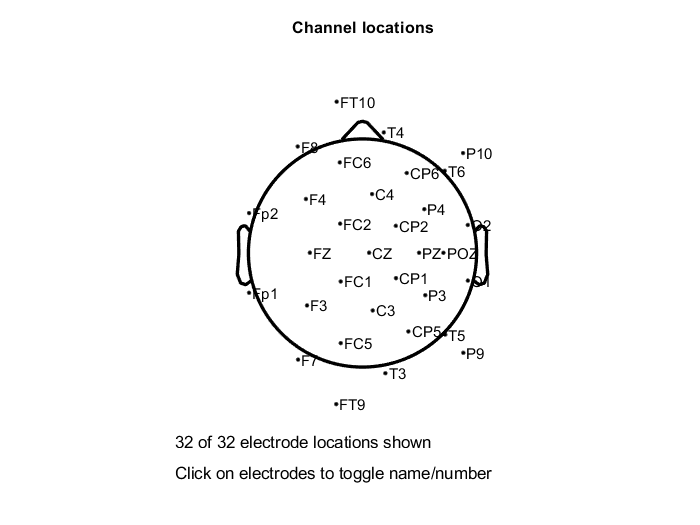
\includegraphics[width=\textwidth]{Fig/chanel_locs_data1.png}\label{fig:channelLocsData1}}
    \end{minipage}
    \hfill    
    \begin{minipage}{.5\textwidth}
        \subfloat[data 2]{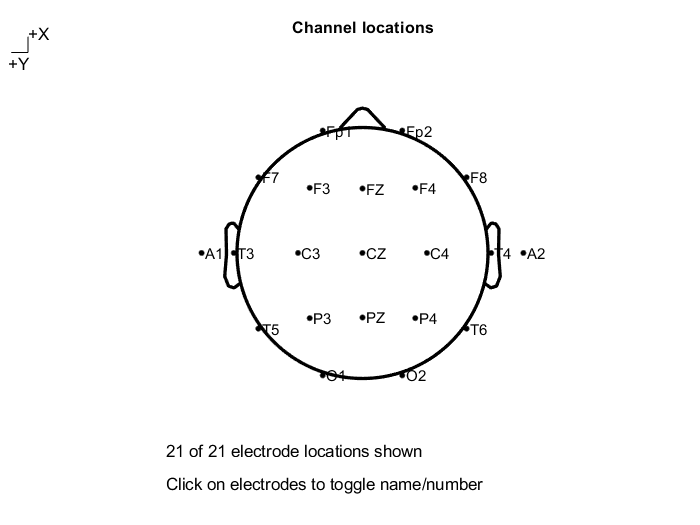
\includegraphics[width=\textwidth]{Fig/chanel_locs_data2.png}\label{fig:channelLocsData2}}
    \end{minipage}
        \caption{Channel Locations}\label{fig:clocs2d}
\end{figure}

\begin{figure}[H]
    \begin{minipage}{.5\textwidth}
        \subfloat[data 1]{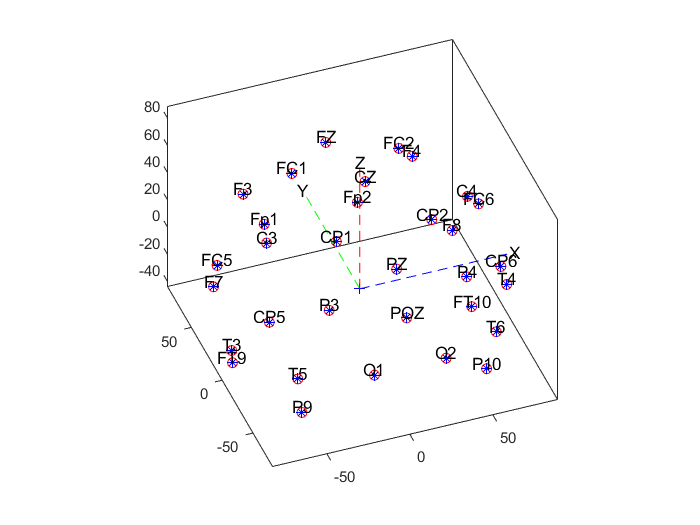
\includegraphics[width=\textwidth]{Fig/chanel_loc_3d_data1.png}\label{fig:channelLocsData1_3d}}
    \end{minipage}
    \hfill    
    \begin{minipage}{.5\textwidth}
        \subfloat[data 2]{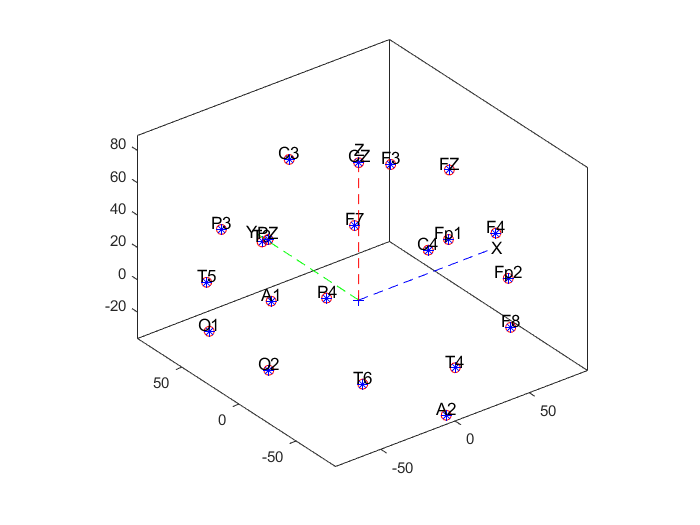
\includegraphics[width=\textwidth]{Fig/chanel_loc_3d_data2.png}\label{fig:channelLocsData2_3d}}
    \end{minipage}
        \caption{Channel Locations 3D view}\label{fig:clocs3d}
\end{figure}

\subsection{High Pass filtering}
here we use a high pass filter with lower band of 1 Hz to cut
baseline drifts(using pop\_eegfiltnew()). \\

\begin{figure}[H]
    \begin{center}
        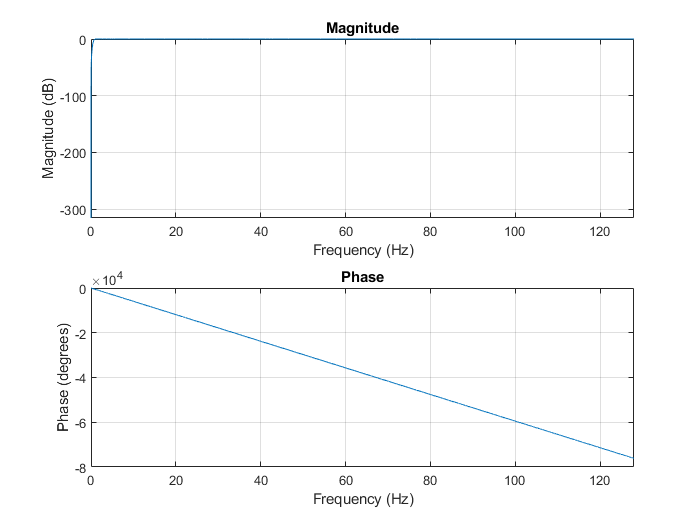
\includegraphics[scale=0.6]{Fig/hpf.png}
        \label{fig:hpf}
        \caption{the high pass filter used}
    \end{center}
\end{figure}

\subsection{Notch line filter}
here we use a notch filter to cut the power line frequency(usually 50 Hz or 60 Hz),
using pop\_cleanline() function. \\
\begin{figure}[H]
    \begin{center}
        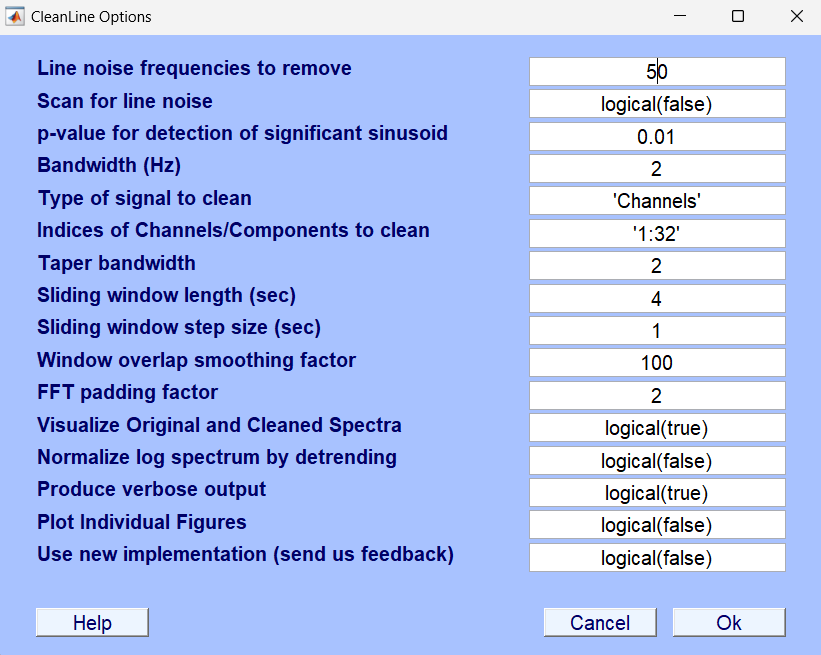
\includegraphics[scale=0.6]{Fig/cleanLine_data1.png}
        \label{fig:cleanLine}
        \caption{Clean Line panel in EEGlab}
    \end{center}
\end{figure}

\subsection{Artifact Removal(and re-referencing)}
first we re-reference the data to the average meaning we take the average 
as the reference for all signals of the electrodes which helps remove the common
noise which may be on all the electrodes using pop\_reref(). \\
then we use pop\_clean\_rawdata() to clean the data of any noises that can be 
detected without ICA such as eye activities or line noises, this method isn't as
effective as ICA but will make the data cleaner for further ICA analysis. \\

\begin{figure}[H]
    \begin{minipage}{.55\textwidth}
        \subfloat[data 1]{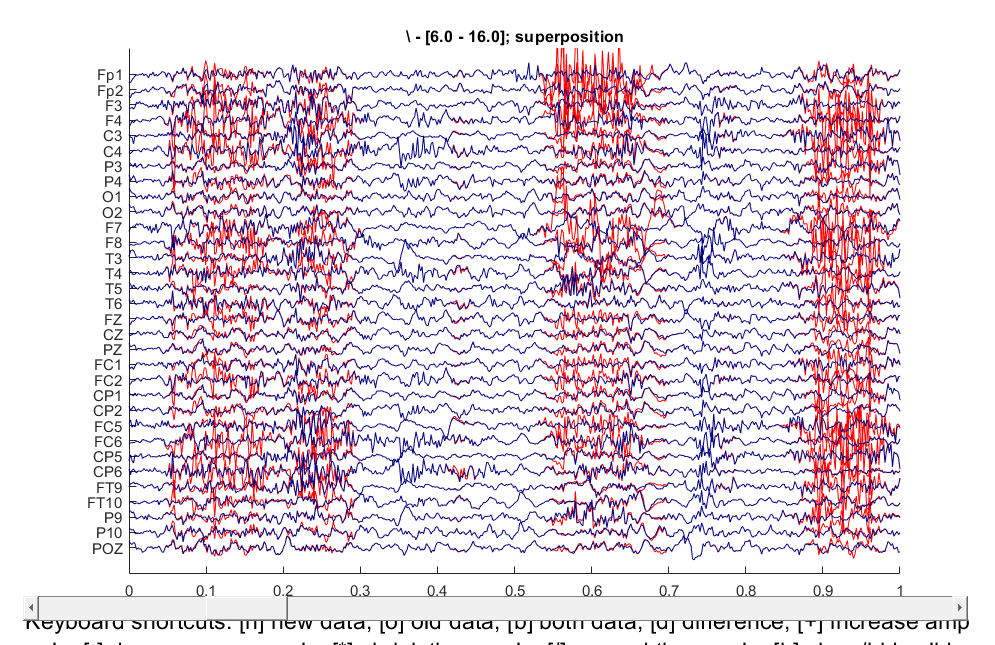
\includegraphics[width=\textwidth]{Fig/ASR_oldNew_data1.png}\label{fig:ASRoldNewData1}}
    \end{minipage}
    \hfill    
    \begin{minipage}{.55\textwidth}
        \subfloat[data 2]{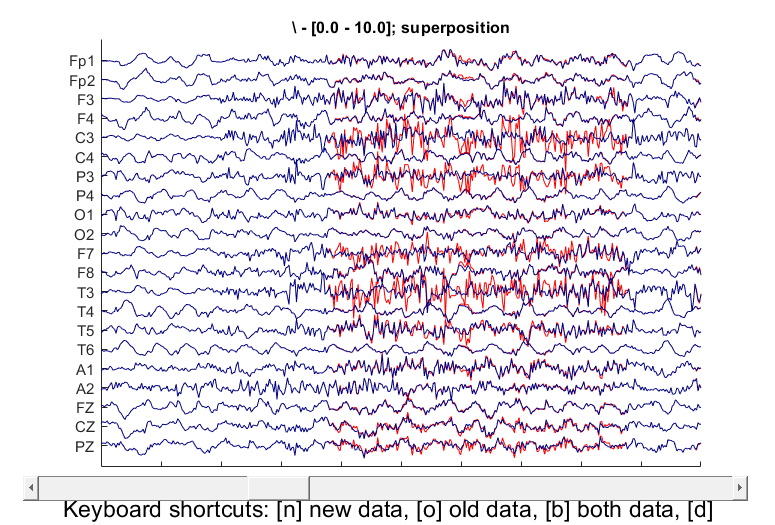
\includegraphics[width=\textwidth]{Fig/ASR_oldNew_data2.png}\label{fig:ASRoldNewData2}}
    \end{minipage}
        \caption{data before and after Artifact removal}\label{fig:clocs3d}
\end{figure}

the we again re-reference the data. \\

\subsection{Independent Component Analysis(ICA)}
Independent Component Analysis(ICA) is a blind source seperation method which
is a way of finding signal sources that are mixed together by analyzing the various 
signals received from different positions.(see the figure below)
\begin{figure}[H]
    \begin{center}
        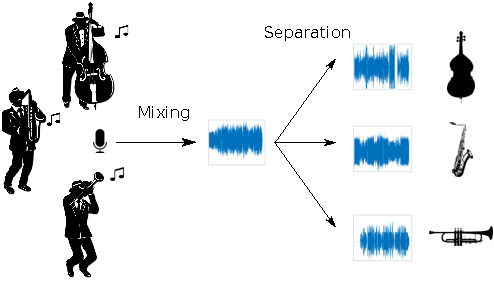
\includegraphics[scale=0.7]{Fig/music_sep.png}
        \label{fig:blindSep}
        \caption{blind source seperation}
    \end{center}
\end{figure}

now using this algorithm we find different components that create the signals
we receive from EEG and then analyze these components by ICA\_label() wich
is trained on brain signals and tries to tell use which signal source is a brain
signal and which are likely noise like muscle, eye blinking or line noise. \\
now using pop\_runica() we start the ICA algorithm: \\
\begin{figure}[H]
    \begin{center}
        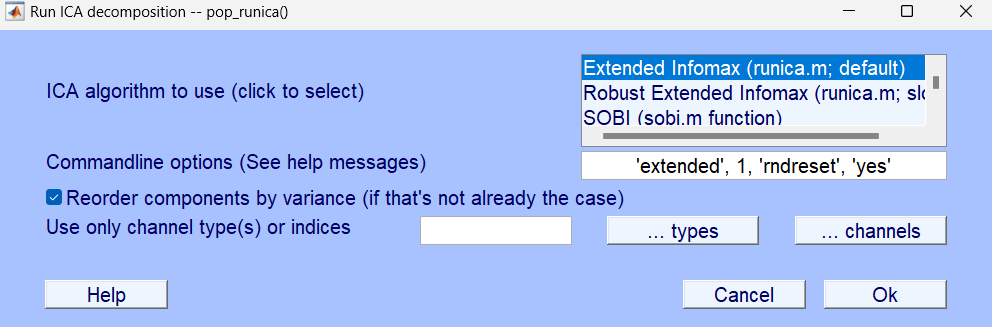
\includegraphics[scale=0.7]{Fig/ICA_data1.png}
        \label{fig:ICA_panel}
        \caption{ICA panel in EEGlab gui}
    \end{center}
\end{figure}

after that we need to give a head model for the dipoles to be fitted to the brain.
using pop\_dipfit\_setting() we fit the MNI model to our brain model to get better results. \\
\begin{figure}[H]
    \begin{center}
        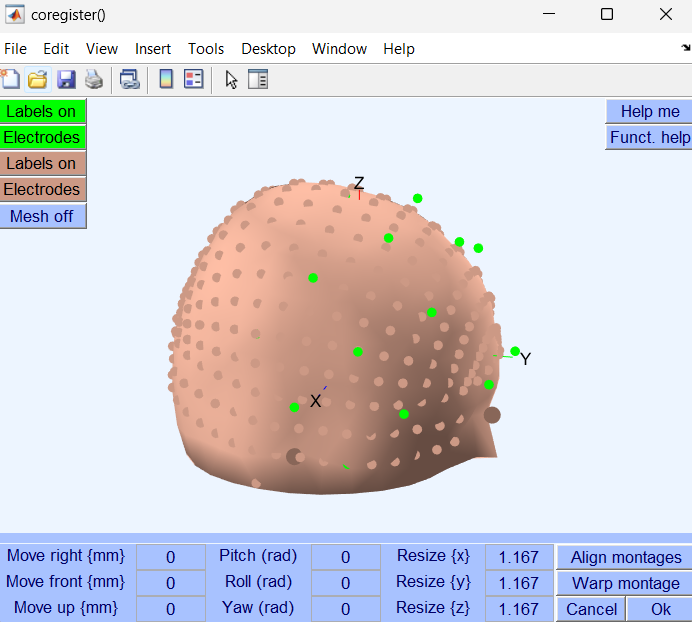
\includegraphics[scale=0.7]{Fig/dipole_fit_coreg_data1.png}
        \label{fig:headmodel}
        \caption{our electrodes before being fitted to the MNI head model}
    \end{center}
\end{figure}

after that we run autofit() in EEGlab that does the br fits the dipoles. \\
then the ICA analysis is ready the ICA components can be seen below: \\

\begin{figure}[H]
    \begin{minipage}{.55\textwidth}
        \subfloat[data 1]{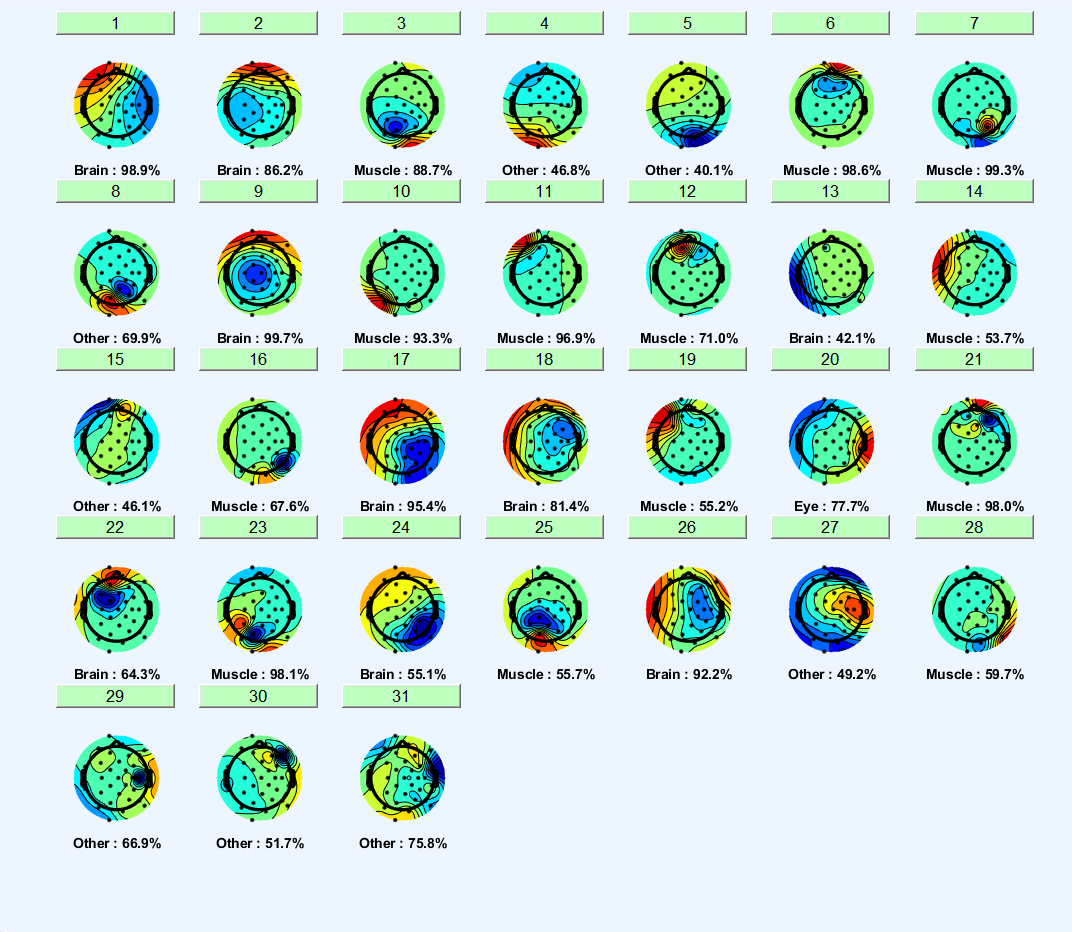
\includegraphics[width=\textwidth]{Fig/ICA_sources_data1.png}\label{fig:sources1}}
    \end{minipage}
    \hfill    
    \begin{minipage}{.55\textwidth}
        \subfloat[data 2]{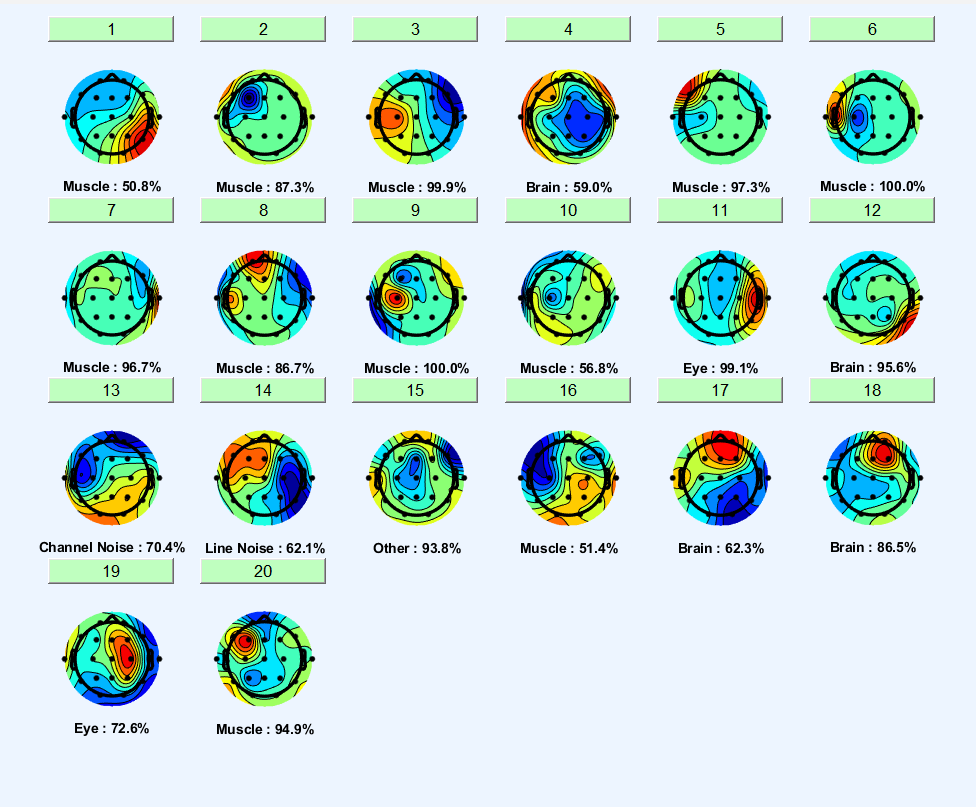
\includegraphics[width=\textwidth]{Fig/ICA_sources_data2.png}\label{fig:sources2}}
    \end{minipage}
        \caption{ICA sources}\label{fig:sources}
\end{figure}

\subsection{Epoching data}
Epoching data is breaking the signals into multiple parts in order to better process them,
a long session of EEG recording can have multiple things happening in them that
should not be processed together, for example if the patient is stimulated at a special
time at the session with one stimulant and at another time with another one we may
want to do different processing(and even pre-processing) on the first and another on
the second signal because of the different nature if the tasks. \\


\subsection{Code}
the code history is presented in a zip file that is alongside this PDF.


\section{Deliverables}
\subsection*{Frequency Spectrum:}
the following figures show FZ channel before and after pre-processing on data 1 and 2. \\
\begin{figure}[H]
    \begin{center}
        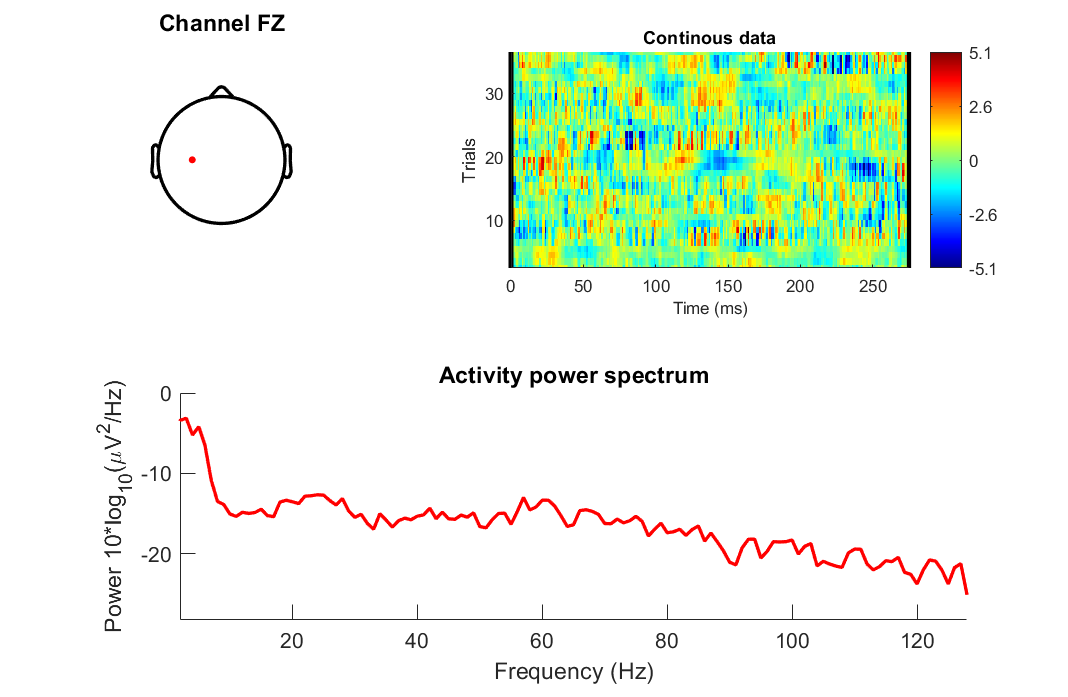
\includegraphics[scale=0.7]{Fig/Fz_spectra_raw_data1.png}
        \label{fig:fzRaw1}
        \caption{data 1 raw FZ channel}
    \end{center}
\end{figure}

\begin{figure}[H]
    \begin{center}
        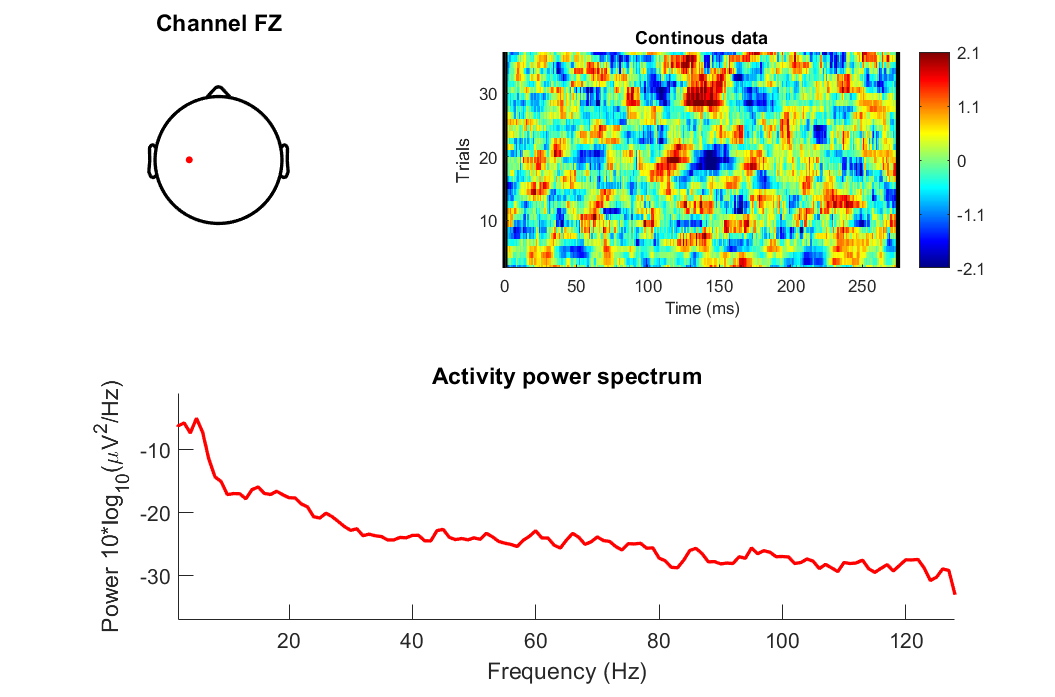
\includegraphics[scale=0.7]{Fig/Fz_spectra_preprocessed_data1.png}
        \label{fig:fzPre1}
        \caption{data 1 pre-processed FZ channel}
    \end{center}
\end{figure}

\begin{figure}[H]
    \begin{center}
        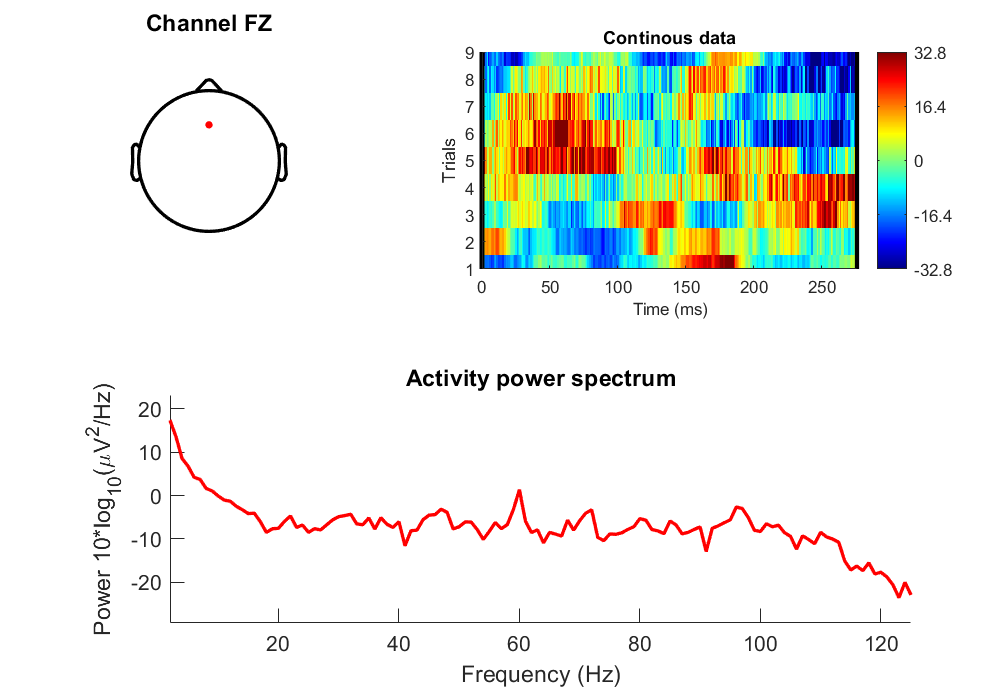
\includegraphics[scale=0.7]{Fig/Fz_spectra_raw_data2.png}
        \label{fig:fzRaw2}
        \caption{data 2 raw FZ channel}
    \end{center}
\end{figure}

\begin{figure}[H]
    \begin{center}
        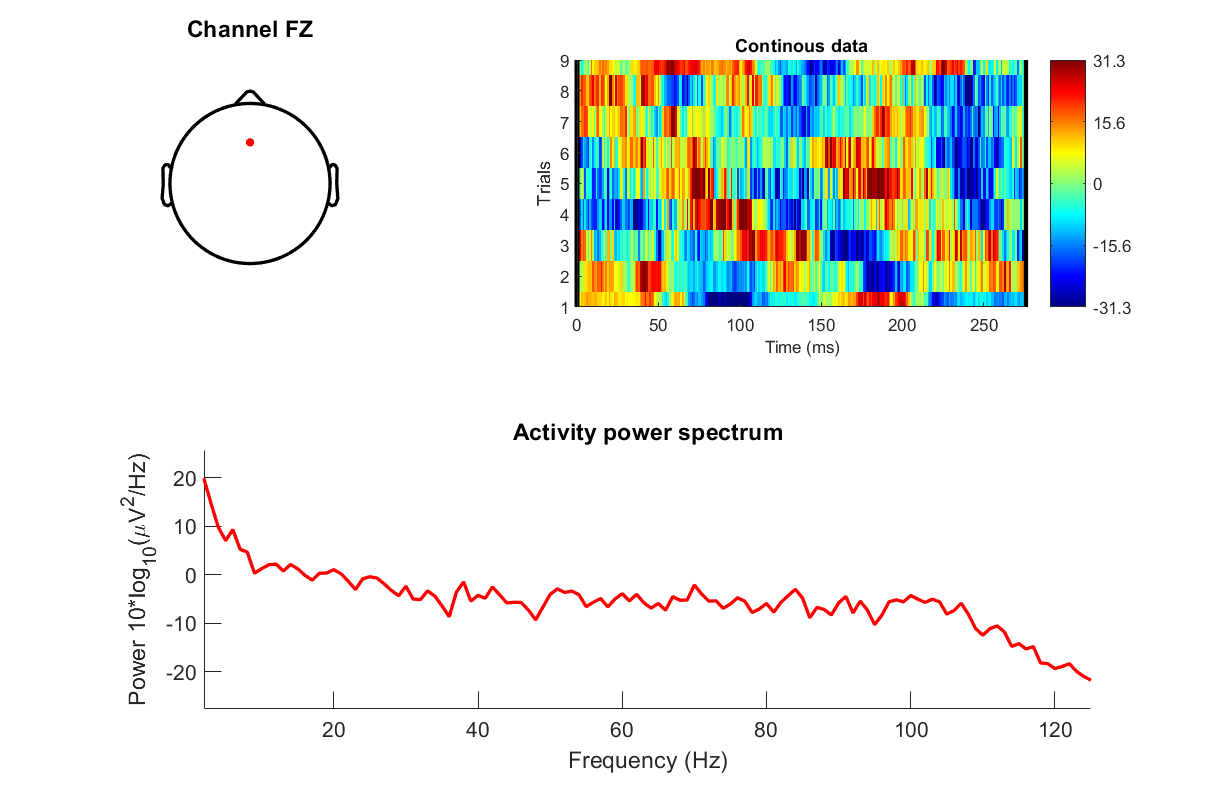
\includegraphics[scale=0.6]{Fig/Fz_spectra_preprocessed_data2.png}
        \label{fig:fzPre2}
        \caption{data 2 pre-processed FZ channel}
    \end{center}
\end{figure}

\subsection*{ICA components:}
here we present one of brain components that are present in each ICA: \\

\begin{figure}[H]
    \begin{center}
        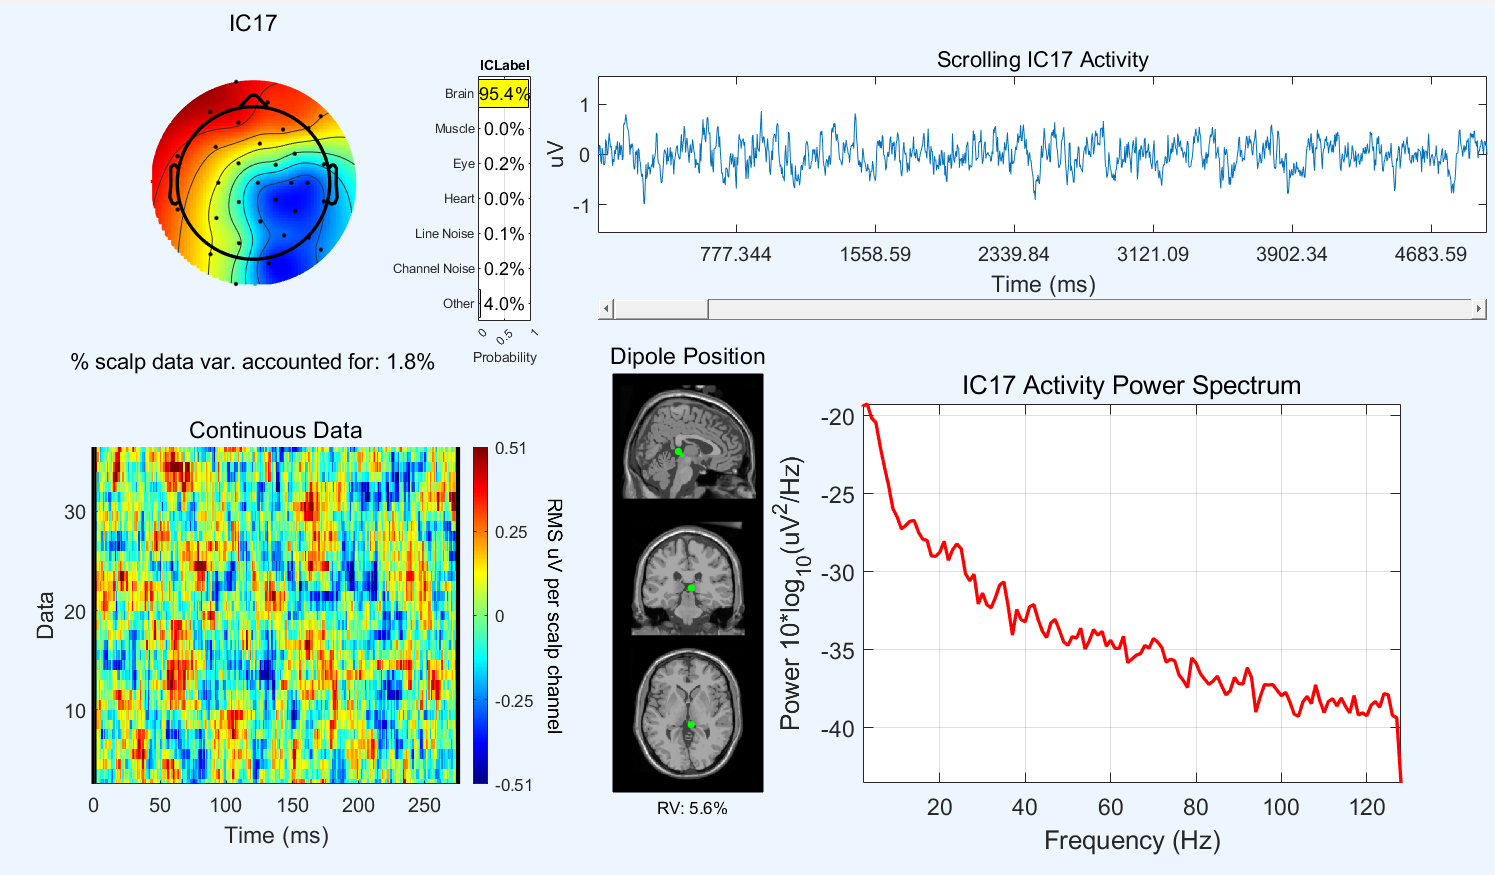
\includegraphics[scale=0.6]{Fig/brain_IC17_data1.png}
        \label{fig:brain1}
        \caption{a brain component from data 1}
    \end{center}
\end{figure}

\begin{figure}[H]
    \begin{center}
        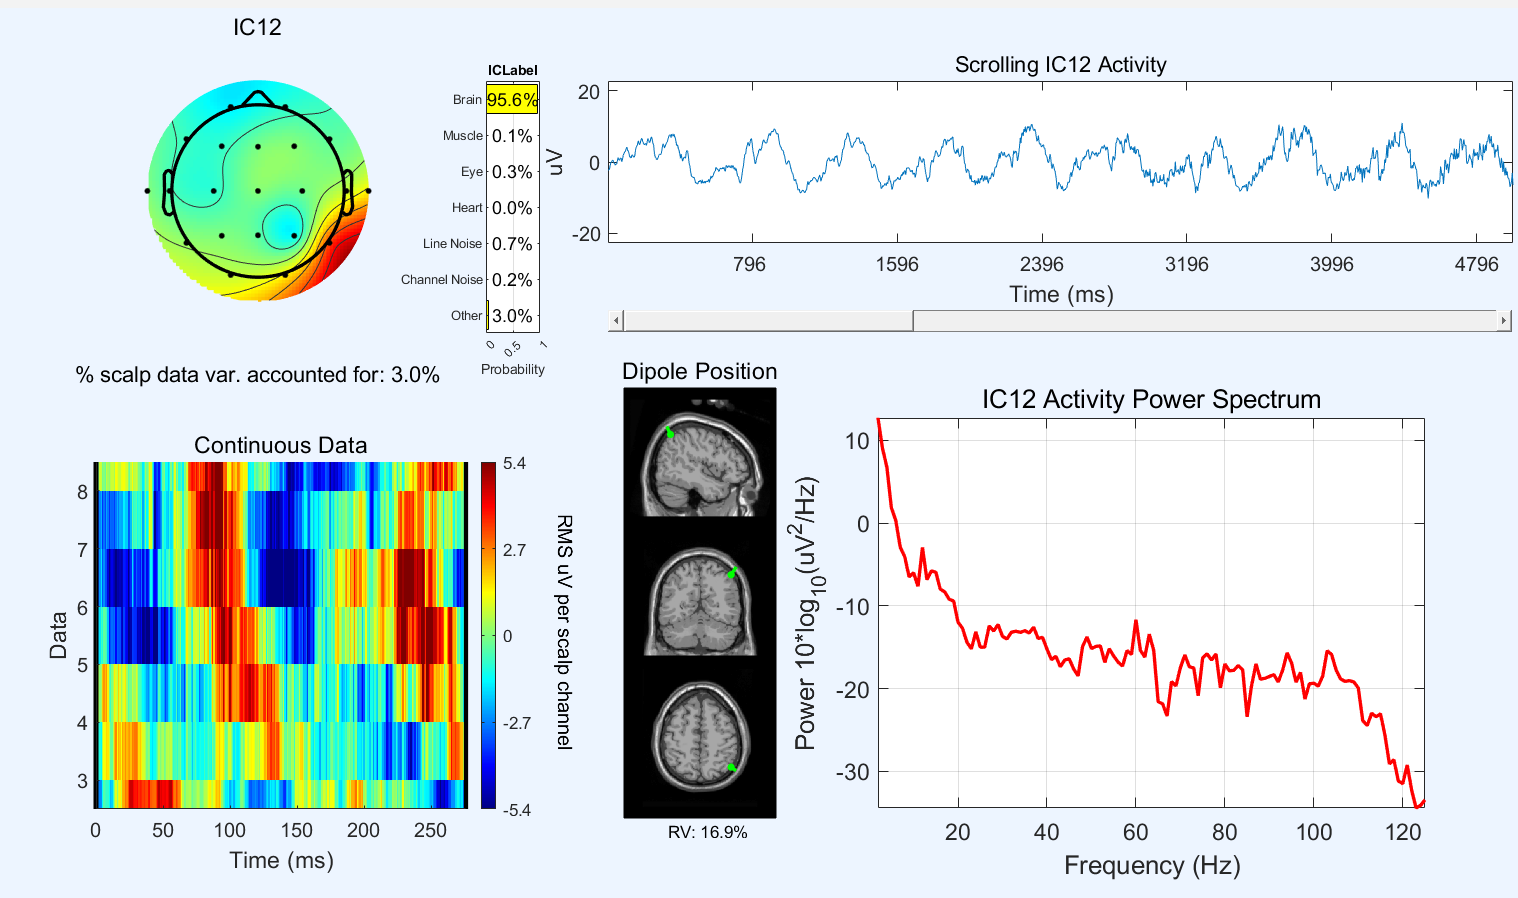
\includegraphics[scale=0.6]{Fig/brain_IC12_data2.png}
        \label{fig:brain2}
        \caption{a brain component from data 2}
    \end{center}
\end{figure}

\subsection{Processed Data}
the processed data is attached in a zip file presented alongside this PDF file. \\
the data is much cleaner and the frequency spectrum resembles a better $\frac{1}{f}$ shape
which we expect a brain signal to be like. the spectrum seems much smoother and it can
be seen that the line frequency which is like a spike atb 60 Hz in data 2 is gone
here are some figures showing the pre-processed data: \\
\begin{figure}[H]
    \begin{center}
        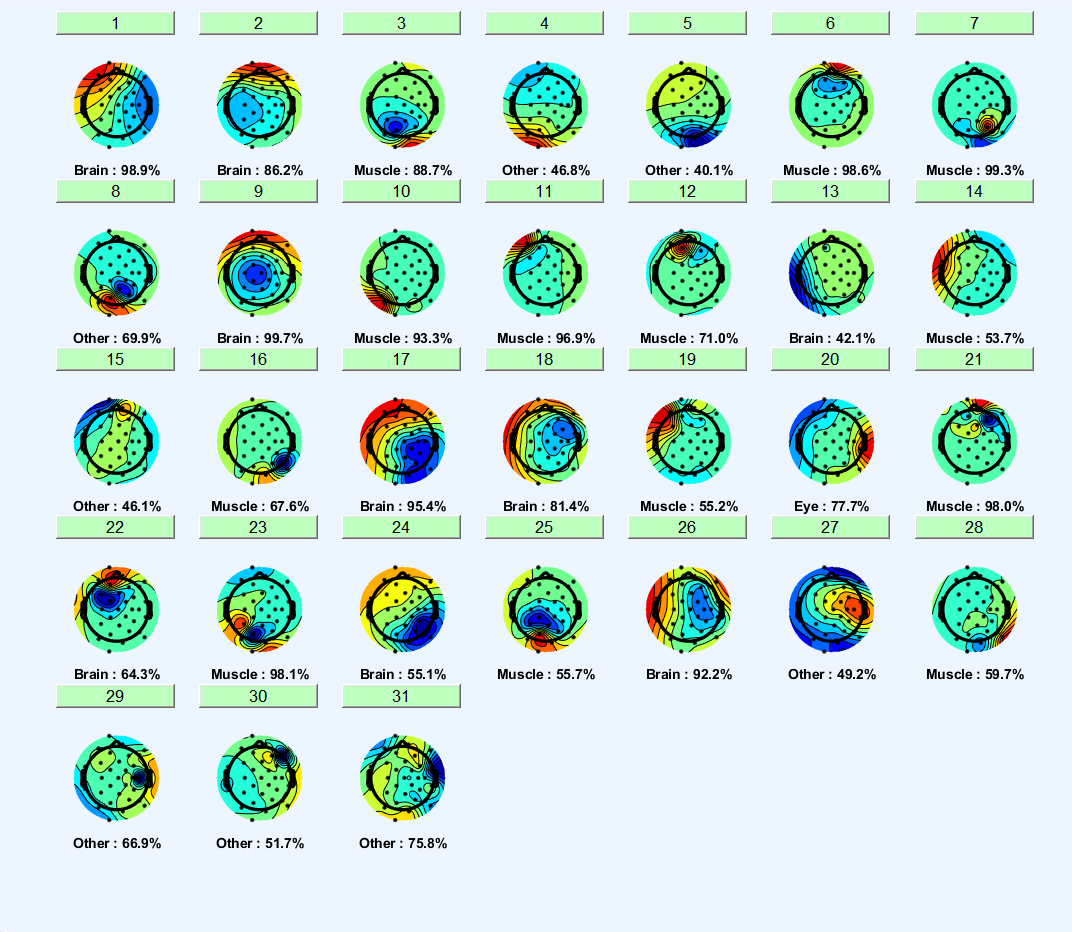
\includegraphics[scale=0.55]{Fig/ICA_sources_data1.png}
        \label{fig:ICAsources1}
        \caption{data 1 ICA}
    \end{center}
\end{figure}

\begin{figure}[H]
    \begin{center}
        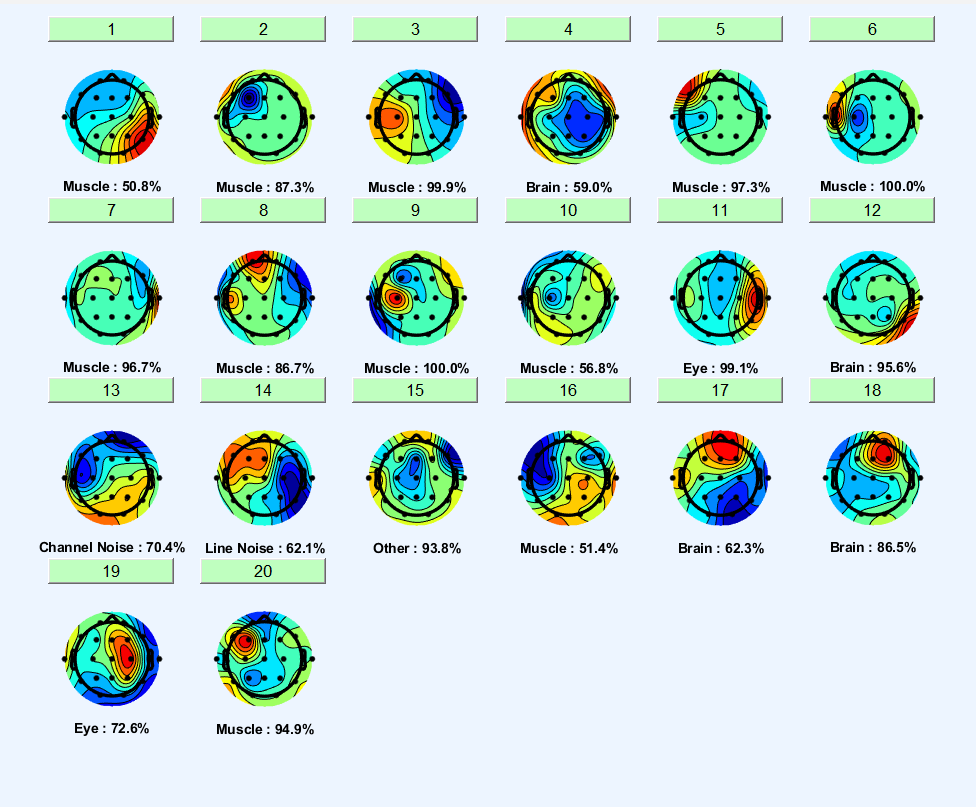
\includegraphics[scale=0.55]{Fig/ICA_sources_data2.png}
        \label{fig:ICAsources2}
        \caption{data 2 ICA}
    \end{center}
\end{figure}


\begin{figure}[H]
    \begin{center}
        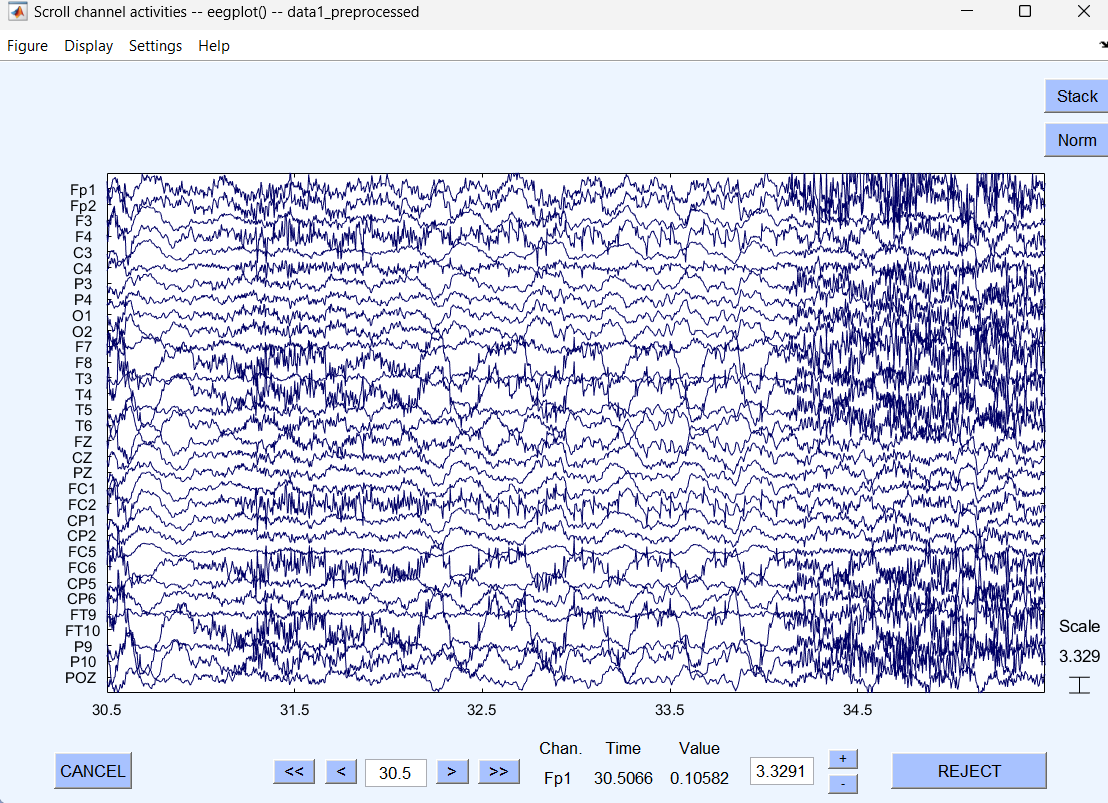
\includegraphics[scale=0.55]{Fig/channel_activity_data1.png}
        \label{fig:data1Activity}
        \caption{data 1 signal after Preprocessing(a change in signal can be seen that is likely the seizure)}
    \end{center}
\end{figure}

\begin{figure}[H]
    \begin{center}
        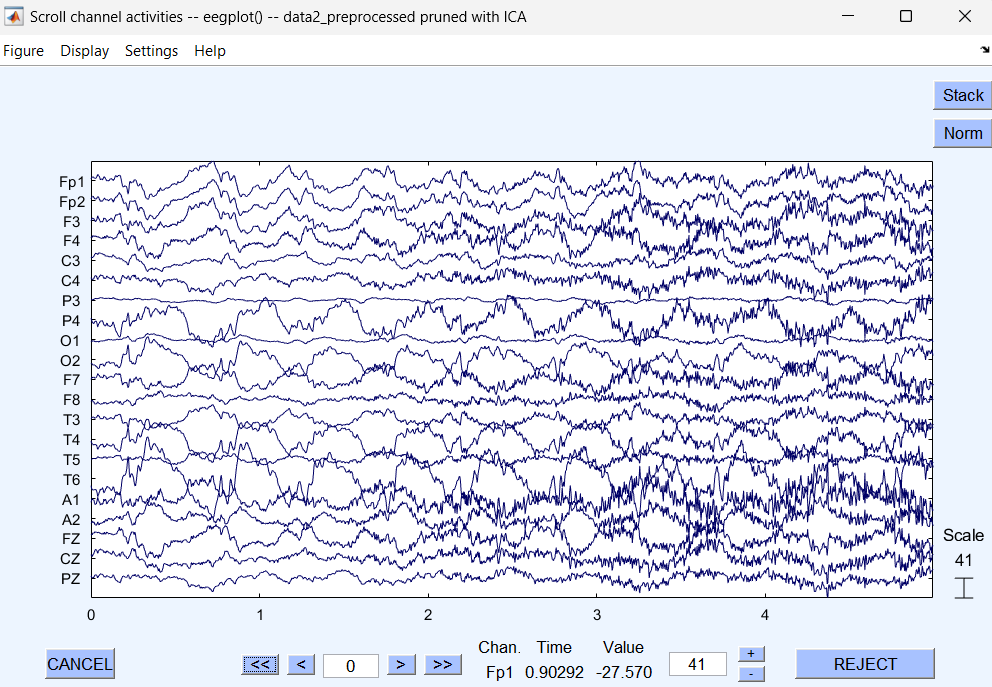
\includegraphics[scale=0.55]{Fig/channel_activity_data2.png}
        \label{fig:data2Activity}
        \caption{data 2 signal after Preprocessing}
    \end{center}
\end{figure}


\end{document}